\chapter{Selection of Third Party Software}
\label{chapter:selection.of.third.party.software}

This chapter will first describe the ingredients in our prototype software
stack. Afterwards we'll account for the tools we've used while developing
this software stack.

Firstly one important aspect with the software used in our thesis work
\dash{}from operating system to third party libraries\dash{}is
that it should only consist of \term{open source}
\sidenote{
  Open source software was introduced as an alternative to
  \term{free software} in the hopes of avoiding confusion and making
  such software more  appropriate for the corporate world
  \citep[p.~7]{fogel05}.
  \work{The Open Source Definition} \citep{osind} dictates the terms
  software needs to follow to be accepted as open source.
}
software. In our experience it's
invaluable to have sources available for all involved software. If one
encounter abnormal behavior or bugs it's much easier to locate them when one
have sources available and one can trivially (depending on the complexity of
the problem) create a patch that sorts them out. One of the motivating factors
of open source contributors is the opportunity for other users to find and fix
failures and provide improvements on their code \citep[p.~87]{hippel05}.

It's also our experience that one can find third party software that fits
one's problem domain more easily if one chooses to use open source software
because of the vast availability of such software.
\citet{deshpande08} found that the availability of open source
code and projects had grown exponentially from January 1995 to December 2006.

Lastly it's of importance to keep the act of conducting science open so that
future researchers easily can discuss, falsify, and improve on previous
research. Software is often an essential part of computer science research and
\citet[p.~430]{kelty05} therefore argues that open source
is a property to strive for when conducting such research.

\section{Prototype Software Stack}

Based on the design and architectural decisions made in 
\chapterref{implementation} we'll now go on to make more fine-grained choices
of what specific third party software components to utilize in our prototype
application. We've decided to harness some of the seemingly best freely
available software components in this software stack. The issue of such code
reuse was introduced by \citet[\pp{138}{142}]{mcilroy68} when he voiced a need
for the software industry to become industrialized. His proposed technique for
enabeling mass-production of software was to offer components\dash{}faimiles
of program routines that can be used for any given job. These components
should be created in a way so that they can fit together as building blocks.
The developer should be able to treat these components as \term{black boxes}%
\evensidenote[-3\onelineskip]{
  In the field of electronics black boxes are used to describe electronic
  circuts with a fixed set of terminals where one is deliberatly ignoring
  the itnernals of the circut. Only the external properties of the circut
  given by the electronic properties of it's terminals are emphasized
  \citep[\p{171}]{wilson79}. Paralelling with computer science we can think of
  a component, module, object, or routine (electornic circut) as beeing a
  black box when we're only concerned by it's input and output characteristics
  trough it's interface (terminals).
}.

After object-oriented programming became the most popular
programming paradigm%
\sidenote{
  According to \abbr{TIOBE}'s list of of
  how popular different programming languages are (based on the number of
  engineers using them, courses given for them, and third party vendors
  endorsing them) 65.463 percent of language use were object oriented
  \citep{tiobe08}.
  The languages counted towards object orientation were: Java, PHP,
  C++, Perl, Python, C\#, Ruby, Delphi, JavaScript, D, FoxPro, Ada, and
  ColdFusion.
}
it's become commonplace to offer software components in the form of classes
and modules which easily can be integrated into a new software project.
As \prequote[\p{37}]{alahmad99}{puts it}{%
  code reuse is what object-orientation [is] all about in the first place}


\subsection{Client-Side}

\subsubsection{Platform}
\label{section:selection.stack.client.platform}

The platform for the clients is in essence a web browser. We are making
changes to a web page after all. The web browser have to be explicitly chosen
to be one that readily supports scripting existing
web pages\dash{}a term often called \term{user scripting}.
The \project{Firefox}%
\sidenote[-3\onelineskip]{
  Available at \url{http://www.mozilla.com/en-US/firefox}.
}
web browser was the first browser providing a
plug-in for handling such scripting of web pages and seems to have the most
mature implementation in our view. Since Firefox also is the
most adopted%
\sidenote{
  According to \citet{onestat08} Firefox was the second most used web browser
  only surpassed by \project{Internet Explorer}.
}
cross-platform open source web browser the platform choice was quite easy.

Firefox provide user scripting trough the means of the
\project{Greasemonkey}%
\sidenote{
  Available at \url{http://greasespot.net}.
}
browser extension. Essentially all it provides is the ability for a user to
install a script which can manipulate the behaviour and properties of an
existing web page using the \term{\abbr{DOM}}%
\sidenote{
  The \abbr{DOM} is a three of objects representing the hierarchical
  structure of nested tags (with text and attributes) in \abbr{HTML}
  documents \citep[pp.~307--310]{flanagan06}.
}.
When a user have such a script for a specific web page installed it's
instructions will be executed on the next visit to the given site, enabling
all kinds of modifications to the \abbr{DOM}.
Some have predicted that Greasemonkey could enable users to
finally \val{take back the Web}\dash{}making the decision of how a web page
behaves and what information it presents the choice of the user of a web page,
not the creator \citep[pp.~3--4.]{filman06}
Although most often used
for customizing the apperance of a given web site \citep[p.~39]{vitali06},
Greasemonkey can also be used for creating new navigational designs on the
\urort{} web site.

Although we've settled on the Firefox and Greasemonkey platform there is a
certain possibility that our implementation could work in other browsers
providing user scripting. The \project{Opera} browser provides user scripting
without any plugins%
\sidenote[-\onelineskip]{
  For more information see
  \url{http://www.opera.com/support/tutorials/userjs/examples}.
},
the \project{Safari} browser can handle user script with the
\project{GreaseKit}%
\sidenote[-\onelineskip]{
  Available at \url{http://8-p.info/greasekit}.
}
plug-in. We have not tested such support for ourselves since we decided to
focus all our efforts on one platform and thereby not be subjected to
cross-browser diffrences\dash{}both in potential bugs and programmatic
interfaces.

\subsubsection{Programming Language}
\label{section:selection.stack.client.language}

The ability to programmatically alter behavior inside web browsers was first
introduced by \project{Netscape} in their 2.0 version of the web browser
with the same name. \project{JavaScript} was first intended to be a
lightweight scripting language for gluing together \abbr{HTML} and applets
written in the \project{Java} programming language \citep{netscape95}.%
\oddsidenote{
  Sun Microsystems, the creators of Java, had negotiated with
  Netscape about including it in their second major web browser release.
  The development of JavaScript, then called Mocha, was already
  underway and people inside Netscape wondered why one needed two
  languages.
  \postquote{eich08}{%
    The answer was that two languages were required to serve the two
    mostly-disjoint audiences in the programming ziggurat who most deserved
    dedicated programming languages: the component authors, who wrote in C++
    or (we hoped) Java; and the `scripters', amateur or pro, who would write
    code directly embedded in HTML}
}
Java applets never took off and JavaScript soon became the \latin{de facto}
standard for enabling behavior on the Web and was standardized as
\project{ECMAScript} in 1997 \citep{ecma99}.

Because of this we had no say in what programming language to use on the
client-side. That is not to say that JavaScript is a poor programming
language. Contradictory to it's name, JavaScript bears few similarities to the
Java language.%
\sidenote{
  The name was more of a marketing decision when Netscape teamed up
  with Sun
  \citep[p.~2]{flanagan06}.
}
Despite it's origins as a scripting language JavaScript is now considered
a full-featured modern programming language
\citedouble{p.~2}{flanagan06}{p.~3}{resig06} including object-orientation.

\subsubsection{Convenience Library}

We decided to use a JavaScript library to make interactions with the
\abbr{DOM} simpler.
In addition there recent JavaScript convenience libraries provide a
unified interface to the browser\dash{}abstracting away inconsistencies
between browser vendors. Lately a myriad of such frameworks have appeared,
but the most interesting ones seems to be
\project{Prototype},
\project{Yahoo! UI Library} (\abbr{YUI} for short),
\project{MooTools},
\project{MochiKit}, and
\project{jQuery}.%
\sidenote{
  Available, in respective order, at
  \url{http://www.prototypejs.org},
  \url{http://developer.yahoo.com/yui},
  \url{http://mootools.net},
  \url{http://mochikit.com}, and
  \url{http://jquery.com}.
}
There are other frameworks available that provide everything but the kitchen
sink but we needed a lightweight or modular solution.

As can be seen in the following table we summarized the size of the most
current version for each library of this writing. These are not exact
metrics\dash{}we selected not to include certain widgets and logging
facilities for the modularized libraries\dash{}but should provide clear
guidance. To keep a level playing feel in this comparison we did not use
minified (removal of comments and unnecessary spaces) or packaged (compressed)
versions of the libraries. All comments and documentation was stripped with a
small script presented in \sourcecodepageref{javascript.comment.sripping}
since the in-line documentation and commenting varied amongst the libraries.

\sidetable{JavaScript Library Comparison
           \label{table:javascript.library.comparision}}{%
  
  \begin{tabular}{lr}

    Library & Size \\
            & (kB) \\
    \midrule

    MooTools (1.11)     & 67 \\
    jQuery (1.2.3)      & 91 \\
    Prototype (1.6.0.2) & 122 \\
    MochiKit (1.3.1)    & 181 \\
    \abbr{YUI} (2.5.0)  & 286 \\

  \end{tabular}
}

We played around a bit with the different libraries to get a feel for how
they worked. What follows is a comparison of simple \abbr{DOM} manipulation
for the different libraries. We followed the official documentation for the
various libraries and tried to solve or problem as succinct and clearly as
possible. We tried to add a \code{class} attribute of \val{highlight} to
all \code{em} elements with an descendant \code{p} element: 

\begin{scode}{Java}{dom.manipulation.prototype}{%
  \abbr{DOM} Manipulation with Prototype}{%
  DOM manipulation in JavaScript with the Prototype library}
\begin{lstlisting}
getElementsBySelector("p em").each(function(em) {
  em.addClassName("highlight");
});
\end{lstlisting}
\end{scode}

\begin{scode}{Java}{dom.manipulation.yui}{%
  \abbr{DOM} Manipulation with Yahoo! \abbr{UI} Library}{%
  DOM manipulation in JavaScript with the Yahoo! UI library}
\begin{lstlisting}
var em = YAHOO.util.Selector.query("p em"); 
YAHOO.util.Dom.setClass(em, "highlight);
\end{lstlisting}
\end{scode}

\begin{scode}{Java}{dom.manipulation.mootools}{%
  \abbr{DOM} Manipulation with MooTools}{%
  DOM manipulation in JavaScript with the MooTools library}
\begin{lstlisting}
$$("p em").each(function(em){
  em.addClass("highlight");
});
\end{lstlisting}
\end{scode}

\begin{scode}{Java}{dom.manipulation.mochikit}{%
  \abbr{DOM} Manipulation with MochiKit}{%
  DOM manipulation in JavaScript with the MochiKit library}
\begin{lstlisting}
var p = getElementsByTagAndClassName("p");
for (i = 0; i < p.length; i++) {
  em = getElementsByTagAndClassName("em","*", p[i]);
  for (j = 0; j < em.length; j++) {
    addElementClass(em, "highlight");
  }
}
\end{lstlisting}
\end{scode}

\begin{scode}{Java}{dom.manipulation.jquery}{%
  \abbr{DOM} Manipulation with jQuery}{%
  DOM manipulation in JavaScript with the jQuery library}
\begin{lstlisting}
$("p em").addClass("highlight");
\end{lstlisting}
\end{scode}

When we compare these rather trivial problem solutions it becomes apparent
that choosing a JavaScript library can have major impact on how easily
implemented and understood your code will be. Four of the five libraries
have support for selector syntax based on
that found in \abbr{CSS}%
\evensidenote{
  Cascading Style Sheets. A stylesheet language for describing the
  presentation of for instance \abbr{HTML} documents.
}.
This is what makes the MochiKit example the most complex one, requiring the
developer to do two queries into the \abbr{DOM} and construct two
loop structures for iterating over the results.
Prototype and MooTools also requires the developer to loop over a single
result set, but the iteration is abstracted into an \code{each} function
making the logic a bit more clearer. Yahoo! \abbr{UI} Library's \abbr{DOM}
functions works on both single elements and collections of
elements\dash{}eliminating the need for an explicit loop structure.
Notice though that the library from
Yahoo! relies heavily on namespacing\dash{}which is a good thing for
interoperability with other libraries\dash{}but can be a bit verbose at times.

The solution written with jQuery provides even more clarity.
Every query into the \abbr{DOM} returns a special jQuery object which means
that one can call methods like \code{addClass} directly on this object
regardless if the jQuery object holds a single or multiple elements.
Also unique to jQuery is the fact that every method call returns a new jQuery
object. This means that one can \term{chain} methods together, expressing
succinctly and clearly what you intend to accomplish with your code. We can
extend our initial problem and add some punctuation inside our \code{em}
element:

\begin{scode}{Java}{jquery.method.chaining}{%
  jQuery Method Chaining}{%
  Chaining multiple methods together in jQuery}
\begin{lstlisting}
$("p em").addClass("highlight").append("!");
\end{lstlisting}
\end{scode}

Based on the minimal file size jQuery provided (only outbested by MooTools)
and it's clear and unique syntax we decided on selecting it as the JavaScript
library for our implementation. It seems others have take jQuery and it's
virtues to hart as many large corporations like Google, Intel, Dell, and
\abbr{BBC} have used it in their public facing offerings.%
\sidenote[-4\onelineskip]{
  For a complete list see \url{http://docs.jquery.com/Sites_Using_jQuery}.
}

\subsection{Server Side}

\subsubsection{Platform}

\subsubsection{Programming Language}
\label{section:selection.stack.server.language}

When doing prototype work it's important that the programming language one
uses is efficient to work with. This means that programmer efficiency is more
important than computational efficiency (a language's native performance).
Since we didn't have time to invest in learning a new language we had to do
with those we knew from before. Of those \project{Ruby}%
\sidenote[-12\onelineskip]{
  Ruby recedes at \url{http://ruby-lang.org}.
},
\project{Python}%
\sidenote[-9\onelineskip]{
  The home of Python is \url{http://python.org}.
}, and
\project{Common Lisp}%
\sidenote[-6\onelineskip]{
  Common Lisp, the prevalent Lisp dialect today, is a standard \citep{ansi96}
  and has many implementations.
  A gateway to this language and it's many implementations can be found
  at \url{http://common-lisp.net}.
}
were the ones with language features that fitted our development process.
All these languages supports multiple programming-paradigms though Common
Lisp is most functional of nature  while Python and Ruby are more
inclined towards object-orientation.

They are all \term{latent typed}%
\sidenote{
  Latent typing ``is a style of typing that does not require (or perhaps even
  offer) explicit type declarations''\citep{wikipedia08latent}.
}
and have quite expressive syntax. This makes for concise source code.
\citet{yegge07} argues that the worst thing that can happens to a code base is
size which often is the result of code bloat. In addition, both Ruby, Python,
and Common Lisp are \term{interpreted} languages%
\sidenote{
  This is only partly true since Common Lisp implementations incrementally
  compile code and extensions or new implementations for Python and Ruby
  implements just-in-time compilers. In both cases the developer
  does not need to explicitly invoke a compile process before using
  a program, therefore resembling interpreted languages.
}.
This means that the programmer don't have to go trough a compilation process
before he can see the results of his labor. When prototyping rapidly it's
quite convenient to make small changes and see the results instantanously.

Disussion of the virtues of different flavors and implementations of
programming languages have been the subject of endless debate.
In the end we think it comes down to
personal preference and making a pragmatic choice for the tool best suited for
the job at hand. If we had to select a programming language based on our list
of candidates based on the languages syntax and posibilities in itself we
would probably have gone with Common Lisp. \citet[p.~27]{foderaro91} have
called it ``the programmable programming language''based on the fact that
program code in Lisp is data and can be manipulated with the same constructs
one are using on data. This makes it immensly powerfull and is the reason why
it's survived for over 50 years \citep[p.~217]{mccarthy78}
and been able to adopt new paradigms in programming as they've appered.
Even though we walue programming efficiency over computational performance,
it should be noted that Common Lisp have been described as the only performant
dynamic language \citep{martin08} compared to statically compiled languages%
\evensidenote{
  In \work{The Computer Language Benchmarks Game} several programming
  languages are pitched against each other in several tests to determine
  their computational performance. As of this writing (April 2, 2008)
  Common Lisp is 1.8 times slower than the fastest language: C++. Python
  and Ruby are respectively 18 and 56 times slower than the leader.
  Updated results can be found at
  \url{http://shootout.alioth.debian.org/gp4/benchmark.php?test=all&lang=all}.
}.

As it turns out, the most important criteria for choosing our implementation
language was it's library support. In the next section we discuss our options
of such libraries or frameworks. Based on our findings there we landed on
Ruby as the language of our server-side implementation.

\subsubsection{Data Extraction Library}

The core library we need is one that handles data extraction from existing
web pages, so called \abbr{HTML} \term{scraping}. While it's possible to
handle such problems with regular expressions, this becomes tedious after a
while. We therefore prefer a special purpose library.

The major deciding factor when we selected the implementation language was
the availability of such a library and it's usefulness. We've already
revealed Ruby as our implementation language and are therefore killing the
suspense. Our data extraction library of choice is called \project{Hpricot}%
\sidenote{
  Hpricot can be obtained from \url{http://code.whytheluckystiff.net/hpricot}.
  A curious note: Hpricot is written by the same person who created
  Hoodwink.d\dash{}our inspiration for a transparent prototype implementation.
}
and makes \abbr{HTML} parsing a blissful endeavor in our opinion.

The Python alternative for web page scraping is \project{Beautiful Soup}.
We were not able to find any libraries specially made for \abbr{HTML} scraping
implemented in Common Lisp. There exists several \term{\abbr{XML}}%
\sidenote{
  Extensible Markup Language. General purpose markup language specification
  that enables implementors to create custom markup languages.
  \abbr{HTML} is not a subset (specified in) \abbr{XML} \citep{w3c99}.
  \term{\abbr{XHTML}} on the other hand, a reformulated version of
  \abbr{HTML}, is a subset of \abbr{XML} \citep{w3c02}.
}
libraries that could handle our tasks, but none as well integrated as
the Ruby and Python options.

To get a feel for the difference between Hpricot and Beautiful Soup we tried
them out on some trivial examples. Under you'll see the listings for one
of these examples. We are trying to find an \code{em} element with a class
of \code{citation}, which have a \code{p} element as it's parent,
in a \abbr{HTML} document contained in the \code{html} object:

\begin{scode}{Python}{parsing.beautiful.soup}{%
  Parsing with Beautiful Soup}{%
  HTML parsing in Python with Beautiful Soup}
\begin{lstlisting}
html('p').content.findNextSiblings('em', 'citation')
\end{lstlisting}
\end{scode}

\begin{scode}{Ruby}{parsing.hpricot}{%
  Parsing with Hpricot}{%
  HTML parsing in Ruby with Hpricot}
\begin{lstlisting}
  html/'p > em.someclass'
\end{lstlisting}
\end{scode}

We feel that Hpricot's syntax is much clearer than that of Beautiful Soup.
This could be a personal preference since we've used \abbr{CSS} for a long
time and Hpricot's selector syntax is based on \abbr{CSS} and Xpath, just as
jQuery. Hpricot was in fact initially based on jQuery's selector syntax
\citep{why06}. This means that we can use the same syntax for selectors on the
server and client-side\emph{}a cognitive advantage.

\subsubsection{Data Fetching Library}

Since we've selected Ruby as our development language of choice we used
\executable{open-uri}, part of the standard Ruby library, for fetching
documents over \abbr{HTTP}%
\sidenote{
  Hyper Text Transfer Protocol. The data transfer protocol for the Web.
}.
\executable{open-uri} is trvial to use and integrates nicely with Hpricot:

\begin{scode}{Ruby}{fetching.openuri.parsing.hpricot}{%
  Fetching and Parsing with Hpricot and open-uri}{%
  Fetching a HTML document with \executable{open-uri}
  and parsing it with Hpricot to find the first and
  last name of a hCard Microformat}
\begin{lstlisting}
require 'hpricot'
require 'open-uri'

html = Hpricot(open('http://redflavor.com'))
(html/'address.vcard > .fn').inner_html
# => "Eivind Uggedal"
\end{lstlisting}
\end{scode}


\subsubsection{\abbr{JSON} Web Framework}

A web framework or rather \abbr{HTTP}
framework is needed to make the
collected data available for our client. Since we'll only be serving requests
for our JavaScript based client implementation we found it sound to transfer
this data as \abbr{JSON}%
\sidenote{
  \abbr{JSON}, short for JavaScript Object Notation, is specified in
  \abbr{RFC} 4627 \citep{crockford06b}. Shortly put it's a lightweigh data
  interchange format based on the object literals of JavaScript.
}.
Luckily for us there exists a framework for Ruby for handeling such tasks
called \project{Halcyon}%
\sidenote{
  Halcyon can be found at \url{halcyon.rubyforge.org}.
}.
This framework makes the process of developing a web application for serving
\abbr{JSON} requests quite easy. It builds on \project{Rack}%
\sidenote{
  Rack is available at \url{rack.rubyforge.org}.
},
a web server interface that sits between a web framework and a web server. By
using Rack we can easily swap between different web servers that support the
protocoll mandated by Rack's interface layer. To demonstate the simplicity of
this framework we'll show how a simple greeting application could be
implemented:

\begin{scode}{Ruby}{halcyon}{%
  Hello World with Halcyon}{%
  A simple hello world application with Halcyon}
\begin{lstlisting}
class Hello < Halcyon::Server::Base
  route {|r| r.match('/').to(:action => 'greet') }
  
  def greet
    msg = {:interjection => 'hello',
           :noun         => 'world',
           :suffix       => '!'}
    ok(msg)
  end
end
\end{lstlisting}
\end{scode}

What is interesting is that the Ruby \code{msg} key/value hash is serialized
automitically to \abbr{JSON} when a client requests this resource:

\begin{scode}{Java}{halcyon.result}{%
  Client Result with Halcyon}{%
  The result of a client request to the Halcyon hello world application}
\begin{lstlisting}
{"status": 200,
 "body": {"interjection": "hello",
          "noun":         "world",
          "suffix":       "!"}}
\end{lstlisting}
\end{scode}

\subsubsection{Web Server}

Since our web framework builds on Rack we have several web servers to select
from.

% which webserver we selected, and why (mongrel, thin)
% prototype application. load balancing not that important with
% for instance nginx.


\subsubsection{Persistance Library}

We decided to use an \abbr{ORM}%
%\sidenote{
  % define
%}
for abstracting our persistance handeling. With such a solution we could
change relational database engines transparently if  neccesary. In addition
\abbr{ORM} libraries often provide a nice interface to the database
eliminating the need for constructing complex \abbr{SQL}.%
%\sidenote{
  % define
%}.
The most popular \abbr{ORM} libraries for the Ruby language are%
\evensidenote{
  Available at respectively
  \url{http://rubyforge.org/projects/activerecord},
  \url{http://datamapper.org}, and
  \url{http://sequel.rubyforge.org}.
}:

\begin{items}
  \iterm{ActiveRecord} %describe
  \iterm{DataMapper} % describe
  \iterm{Sequel} %describe
\end{items}

\subsection{Overview of Client \oldand Server Components}

With all the pieces in place of our third party software puzzle
we present a high level view of the architecture, from the client to the
server, in
\figureref{fig.prototype.architecture}.

\begin{figure}
  \begin{whole}
    \centering
    \includegraphics[width=0.9\wholewidth]{fig_prototype_architecture}
    \caption[Prototype Architecture]{
      High level view of the overall prototype architecture.
    }
    \label{figure:fig.prototype.architecture}
  \end{whole}
\end{figure}


\section{Development Tools}

As with the implementation platforms, languages, and third party libraries
our first criterion for selecting development tools is freedom.

\subsection{Version Control}

We've found it indispensable to use \term{version control} when writing code
and even used it when authoring this thesis. We'll not spend time to discuss
the merits of version control since we feel it's benefits are major and
using one induces almost zero overhead in your working process. Sometimes we
feel that the use of version control can guide you when conducting complex
tasks.

There are however several different forms of version control system one can
use. One of the most used version control implementations the last years
in open source circles was
\project{Subversion}%
\sidenote[-8\onelineskip]{
  Available at \url{http://subversion.tigris.org}.
}\dash{}a \term{centralized version control system} meaning that one central
server holds the version controlled code repository and it's history.%
\sidenote[-7\onelineskip]{
  Developers on the client-side have working copies and need to contact the
  centralized server to get a hold of historical data and create new history.
}
Recently \term{decentralized version control systems} have become more popular
amongst developers. A decentralized model means that every developer can have
their own repository consisting of all history.%
\sidenote[-5\onelineskip]{
  You can for instance be without internet connectivity and still commit
  changes, revert to previous versions, and handle all other tasks your
  version control system supports.
}
Code is then shared either in a push or pull fashion between such individual
repositories. This enables a much better model for collaboration.
We favor this last model of version control and so have projects
like \project{Linux}, \project{X}, \project{Mozilla},
and \project{OpenSolaris}.%
\sidenote[-3\onelineskip]{
  \citeauthor{torvalds07}, author of the Linux kernel,
  have described Subversion and centralized version control
  as fundamentally flawed since it's supposed to be a
  \q{\abbr{CVS} done right}. Since he feels \abbr{CVS} is flawed Subversion
  is therefore inherently flawed \citeyearpar{torvalds07}.
}

Based on criteria of performance and current adoption there are in our view
only two interesting decentralized version control systems:
\project{Git}%
\sidenote{
  Available at \url{http://git.or.cz}.
}
and \project{Mercurial}%
\sidenote{
  Available at \url{http://www.selenic.com/mercurial}.
}. Both are unique in that they don't track meta-data, they just track
content and meta-data are thereby inferred from the content.
At a very high level view Mercurial have a better user interface and Git
supports some advanced features the former don't have. We opted to used
Mercurial for this development project since we've substantial experience in
using it and did not need any of Git's advanced features.

\subsection{Editor}

A developer's main tool for authoring software is his editor. Sometimes the
language of implementation warrants a specialized editor with aids for
handling cumbersome tasks specific to that language. Such an editor is often
called an \abbr{IDE}%
\sidenote[-7\onelineskip]{
  A good example of an \abbr{IDE} (integrated development environment
  for short) is \project{Eclipse} (available at \url{http://eclipse.org}).
  It was first used for Java development but since extended with
  plugins for handling other programming languages and families.
}
and are used most often for languages like Java and C\#.
\citet{murphy06} found that developers mostly use an \abbr{IDE} for navigating
large collections of source code, refactoring code, debugging code, and
interacting with revision control systems in addition to normal editor usage.
Development environments found in Lisp%
\sidenote[-4\onelineskip]{
  \prequote[p.~69]{sandewall78}{%
    describes the nature and benefits of the Lisp environment as}{%
      The `residential' design of programing systems, whereby all facilities
      for the user are integrated into one system with which the user
      communicates during the entire interactive session, offers great
      possibilities for user convenience}
}
and Smalltalk%
\sidenote{
  Similar to Lisp's programming environment
  \postquote[p.viii]{goldberg83}{%
    Smalltalk is designed so that every component in the system that is
    accessible to the user can be presented in a meaningful way for
    observation and manipulation}

}
are surpassing \abbr{IDE} types in integration and interactiveness even though
they preceded them.

The programming languages we previously settled on, JavaScript and Ruby,
are very expressive and dynamic in their nature in addition to being
interpreted instead of compiled. Our experience is that \abbr{IDE} usage for
such languages stands more in the way than aid you as a programmer during
your problem solving process.
\citet{bray07} conducted a rather unscientific survey of 1000 Ruby
programmers. Despite of the surveys shortcomings it showed that
the majority of Ruby programmers used non-\abbr{IDE} editors for their
development.

The interactive experience provided by Lisp and Smalltalk implementations are
sadly missing%
\sidenote{
  Ruby has an interactive interpreter similar to those found in Lisp and
  Smalltalk environments called \executable{irb}. It's not integrated into an
  overall programming environment and therefore is mostly used for testing out
  small ideas.
}
from JavaScript and Ruby implementations. This means that we're left with
finding a good editor which enables us to focus on writing code as efficiently
and safely as possible. Editor selection is highly a matter of preference and
finding one that matches your work process. Powerful editors have a
reputation of being quite hard to learn. But if you get over the steep
learning curve the benefits the editor gives you are worth it.

\begin{fullquote}{orenstein08}{%
  have experienced how much effort programmers can
  invest in something seemingly trivial as an editor}
    If the thought of switching editors doesn't fill you with quite a bit of
    dread, what you're using now is almost certainly under powered, and you
    definitely haven't customized it enough.
\end{fullquote}
